\documentclass[11pt, oneside]{article}   	% use "amsart" instead of "article" for AMSLaTeX format
\usepackage{geometry}                		% See geometry.pdf to learn the layout options. There are lots.
\geometry{letterpaper}                   		% ... or a4paper or a5paper or ... 
%\geometry{landscape}                		% Activate for for rotated page geometry
%\usepackage[parfill]{parskip}    		% Activate to begin paragraphs with an empty line rather than an indent
\usepackage{graphicx}				% Use pdf, png, jpg, or eps� with pdflatex; use eps in DVI mode
								% TeX will automatically convert eps --> pdf in pdflatex		
\usepackage{amssymb}
\graphicspath{{/Users/telliott_admin/Dropbox/Tex/png/}}

\title{Law of Sines}
%\author{The Author}
\date{}							% Activate to display a given date or no date

\begin{document}
\maketitle
%\section{}
%\subsection{}
\setlength{\parskip}{2 mm}
\large
Here, I will go through algebraic proofs of the Pythagorean Theorem and the Law of Sines.  In the triangle below, A, B, and C are the angles, with side lengths a, b, and c.
\begin{center}
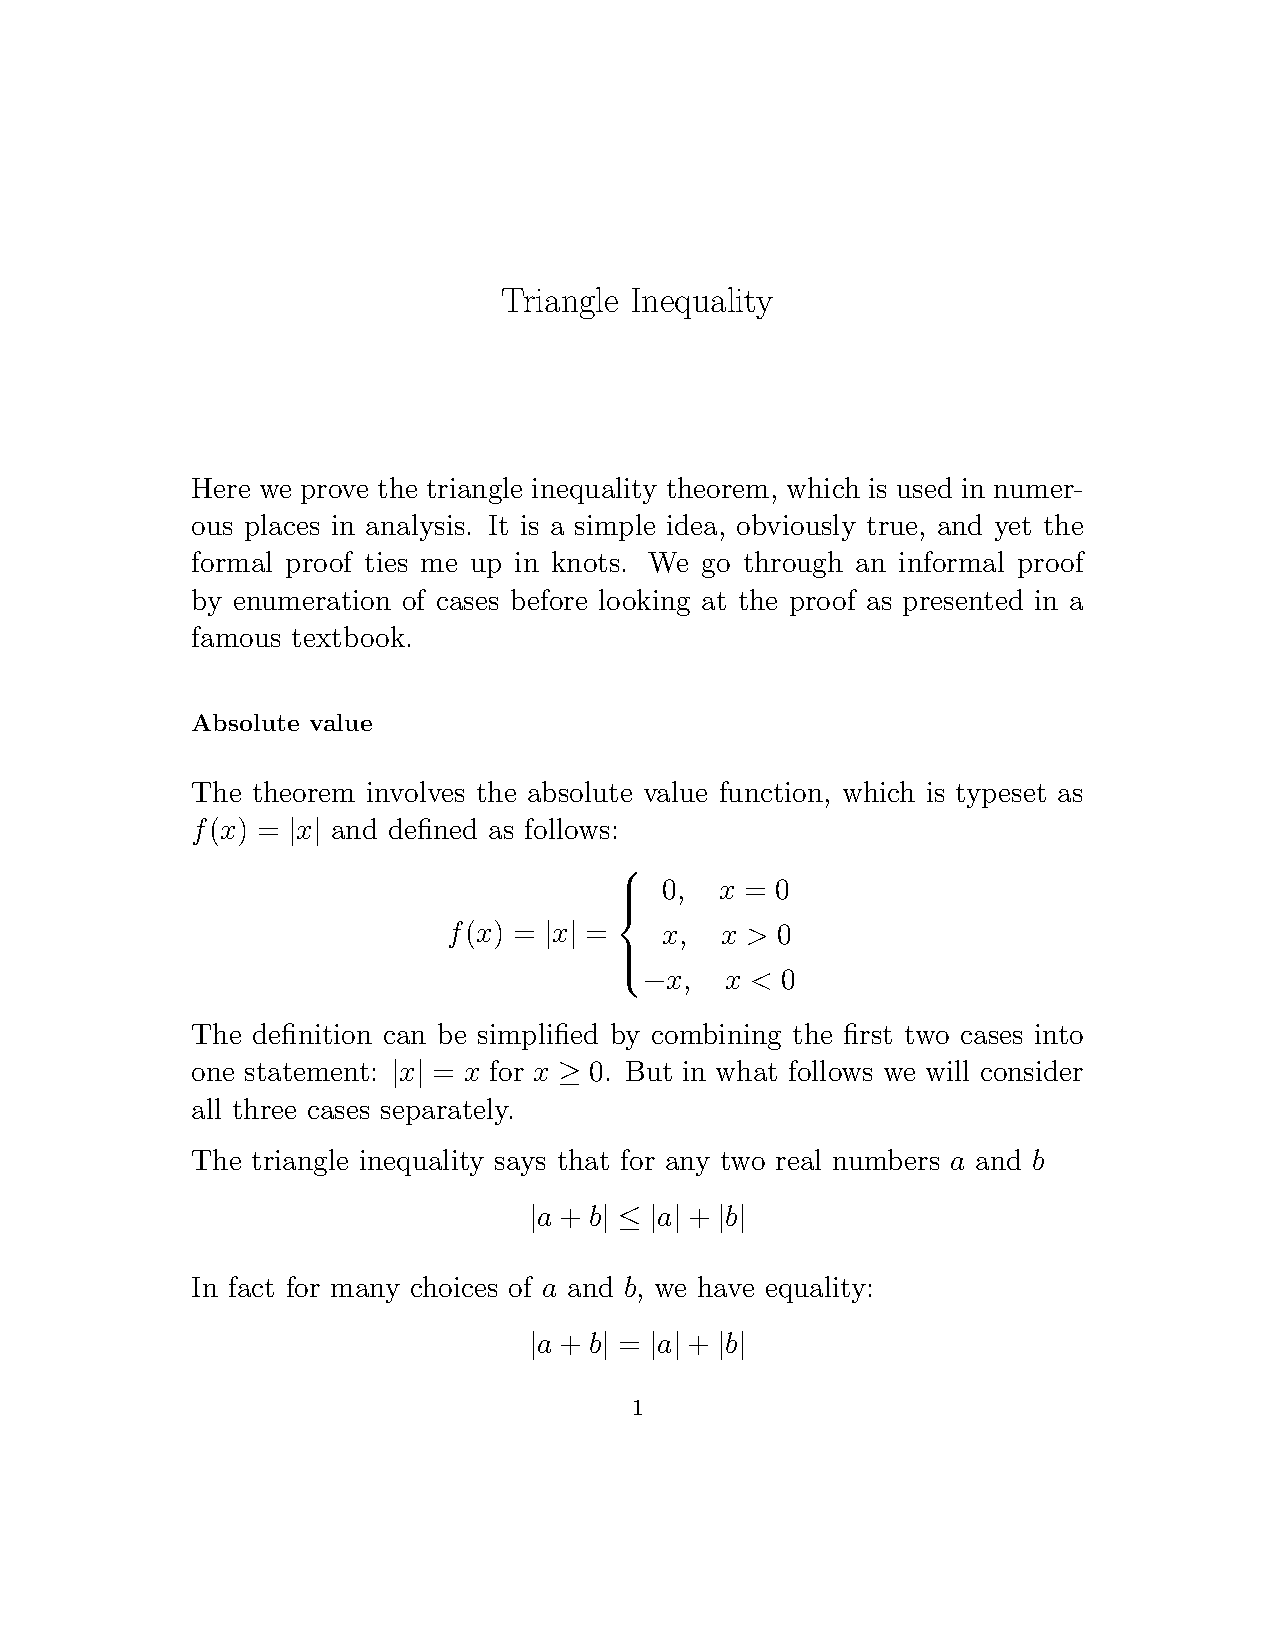
\includegraphics [scale=0.5] {triangle.png}
\end{center}
An altitude has been drawn from angle C to side c opposite.  The altitude is perpendicular to the side c, which is thereby divided into lengths d and e.

Suppose angle C is a right angle.  (I know it doesn't look exactly right, but allow me to just go with it).  If C is a right angle, A and B are complementary:
\[ A + B = 90^\circ \]
Referring to the small triangle on the left, it's clear that the angle (call it $\theta$) between side b and the altitude h is equal to angle B, because
\[ \theta + A + 90^\circ = 180^\circ = B + A + C \]
where $C = 90^\circ$.  Therefore, the small triangle on the left and $\triangle ABC$ are similar.  By similarity, the sides opposite equal angles are in the same ratio so
\[ \frac{d}{b} =  \frac{b}{c} \]
\[ \frac{h}{b} =  \frac{a}{c} \]
By exactly the same argument, the small triangle on the right is similar to both of these, so we can extend the ratios
\[ \frac{d}{b} =  \frac{b}{c} =  \frac{h}{a} \]
\[ \frac{h}{b} =  \frac{a}{c}  = \frac{e}{a}  \]
We have
\[ a^2 = ce, \ \ \ \ b^2 = cd, \ \ \ \ a^2 + b^2 = ce + cd = c(e+d) = c^2 \]
QED.

This is the Pythagorean Theorem.

Looking at the figure again (from now on angle C will not be equal to $90^\circ$), write a formula for the sine of A and sine of B
\begin{center}
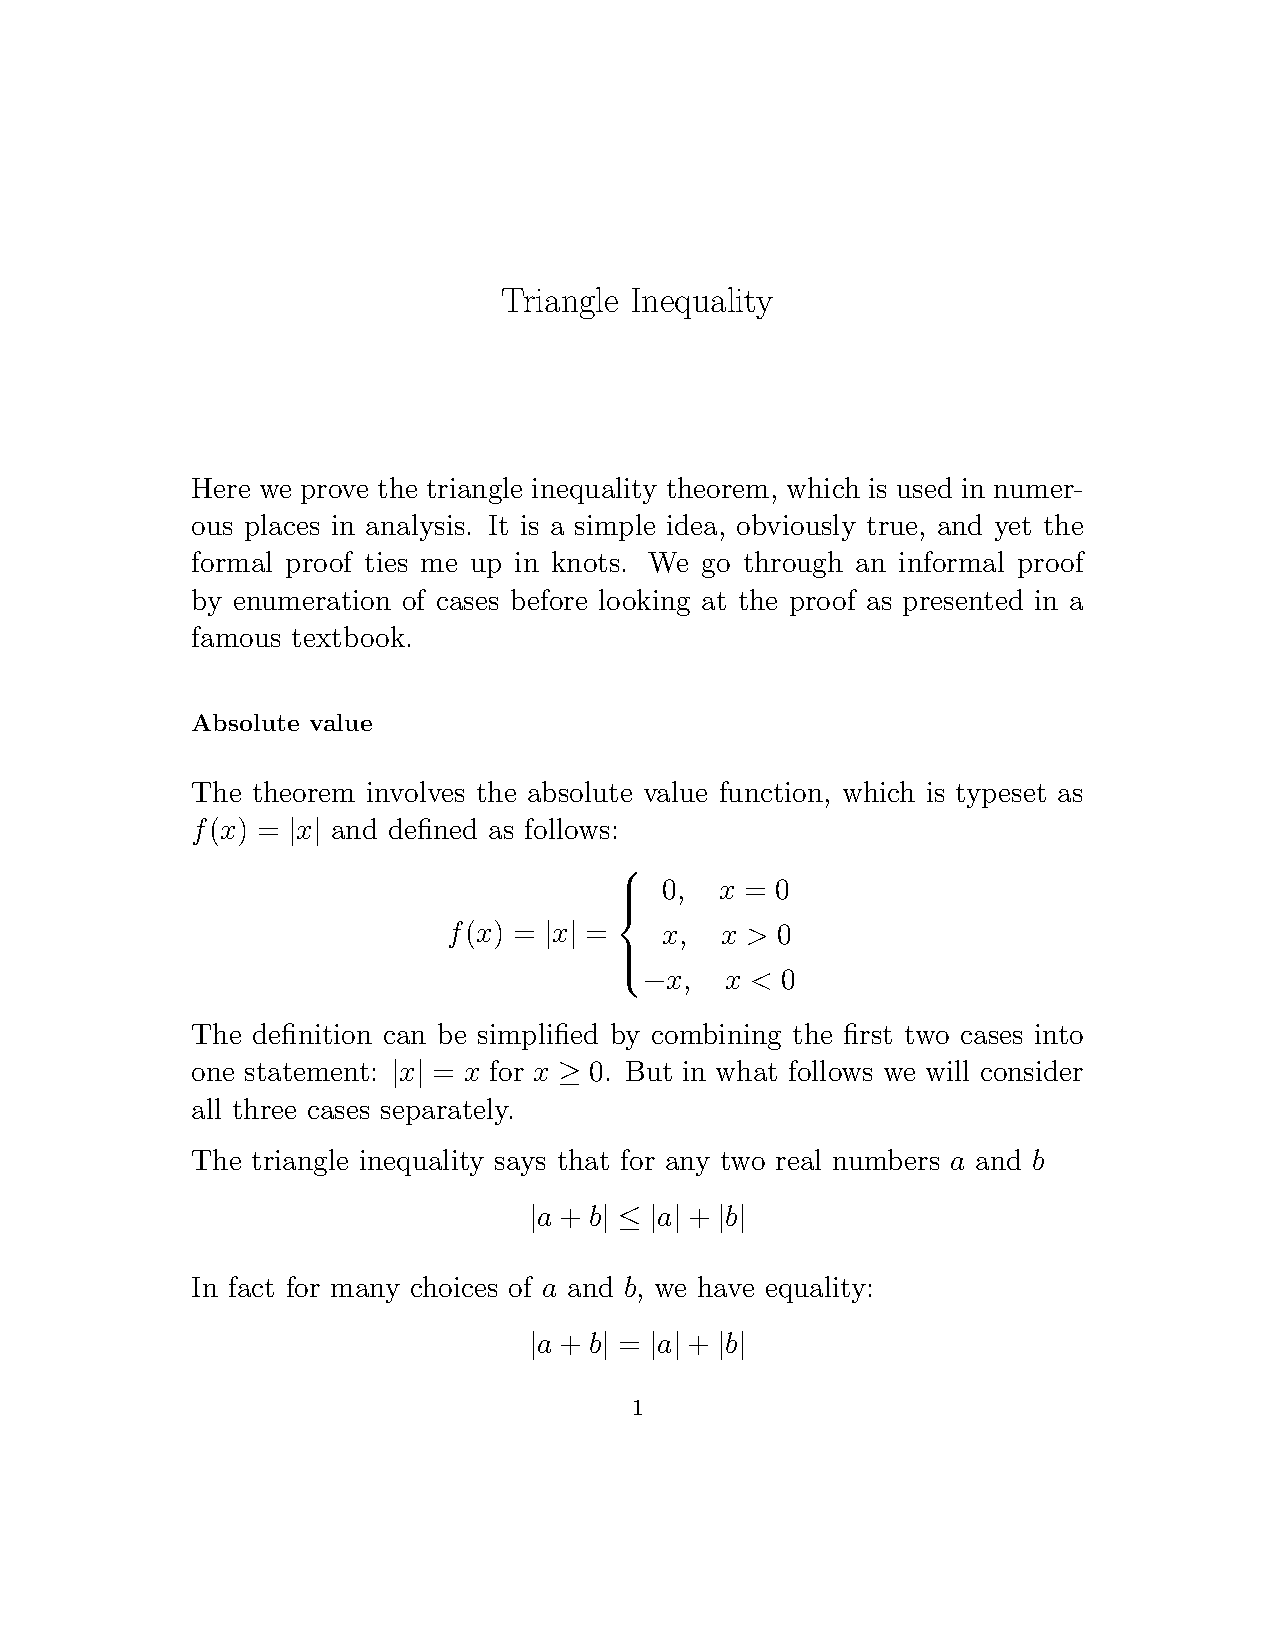
\includegraphics [scale=0.5] {triangle.png}
\end{center}
\[  \frac{h}{b} = sin\ A, \ \ \ \  \frac{h}{a} = sin\ B \]
\[  h = a \ sin\ B  = b \ sin\ A \]
\[  \frac{a}{sin\ A} = \frac{b}{sin\ B} \]
By symmetry, the ratio extends to side c and angle C
\[  \frac{a}{sin\ A} = \frac{b}{sin\ B} = \frac{c}{sin\ C} \]
QED.

We have proved the Law of Sines.

\end{document}  